\appendix
\addtocontents{toc}{\protect\newpage}
\chapter{Generic Programming}
\section{Functor instances for Pattern Functors}
\label{app-inst-functor-patfun}
\begin{minted}{haskell}
instance Functor I where
  fmap f (I r) = I (f r)

instance Functor (K a) where
  fmap _ (K a) = K a

instance Functor U where
  fmap _ U = U

instance (Functor f, Functor g) => Functor (f :+: g) where
  fmap f (L x) = L (fmap f x)
  fmap f (R y) = R (fmap f y)

instance (Functor f, Functor g) => Functor (f :*: g) where
  fmap f (x :*: y) = fmap f x :*: fmap f y
\end{minted}

\chapter{Cache Management}
\section{Implementation Recursion Depth}
\label{app-sec-impl-rec-depth}
\begin{minted}{haskell}
class HasDepth f where
  depth :: f (AFix g MemoInfo) -> Int

instance HasDepth (K a) where
  depth _ = 1

instance HasDepth U where
  depth _ = 1

instance HasDepth I where
  depth (I x) = let ph = getHasDepth (getAnnotation x) in 1 + ph

instance (HasDepth f, HasDepth g) => HasDepth (f :+: g) where
  depth (L x) = depth x
  depth (R x) = depth x

instance (HasDepth f, HasDepth g) => HasDepth (f :*: g) where
  depth (x :*: y) = max (depth x) (depth y)

instance (HasDepth f) => HasDepth (C c f) where
  depth (C x) = depth x
\end{minted}

\chapter{Results}

\section{Minimum of 10 recursion depth}
\label{app-sec-10-rec-depth}
\begin{figure}[H]
  \begin{minipage}{.5\textwidth}
    \centering
    \includegraphics[width=\textwidth]{plots/run-5/time/Worst/10/all_benchmarks.pdf}  
  \end{minipage}
  \begin{minipage}{.5\textwidth}
    \centering
    \includegraphics[width=\textwidth]{plots/run-5/time/Average/10/all_benchmarks.pdf}  
  \end{minipage}
  \begin{center}
    \begin{minipage}[c]{.5\textwidth}
      \centering
      \includegraphics[width=\textwidth]{plots/run-5/time/Best/10/all_benchmarks.pdf}  
    \end{minipage}
  \end{center}
  \caption{The execution time over 10 executions for the Worst, Average and Best case, where the minimum recursion depth is 10.}
\end{figure}
\begin{figure}[H]
  \begin{minipage}{.5\textwidth}
    \centering
    \includegraphics[width=\textwidth]{plots/run-5/memory/Worst/10/all_benchmarks.pdf}  
  \end{minipage}
  \begin{minipage}{.5\textwidth}
    \centering
    \includegraphics[width=\textwidth]{plots/run-5/memory/Average/10/all_benchmarks.pdf}  
  \end{minipage}
  \begin{center}
    \begin{minipage}[c]{.5\textwidth}
      \centering
      \includegraphics[width=\textwidth]{plots/run-5/memory/Best/10/all_benchmarks.pdf}  
    \end{minipage}
  \end{center}
  \caption{The max-bytes-used over 10 executions for the Worst, Average and Best case, where the minimum recursion depth is 10.}
\end{figure}


\newcommand{\individualbenchmark}[2]{
  \begin{minipage}{.5\textwidth}
    \centering
    \includegraphics[width=\textwidth]{#1}
    \caption{#2}
  \end{minipage}
}

\newcommand{\trendlinebenchmark}[2]{
  \begin{figure}[H]
    \individualbenchmark
      {plots/run-3/time/#1/10/#2/cata_sum.pdf}
      {Execution Time - Cata Sum}
    \individualbenchmark
      {plots/run-3/time/#1/10/#2/generic_cata_sum.pdf}
      {Execution Time - Generic Cata Sum}  
  \end{figure}
  \begin{figure}[H]
    \individualbenchmark
      {plots/run-3/time/#1/10/#2/incremental_cata_sum.pdf}
      {Execution Time - Incremental Cata Sum}
    \individualbenchmark
      {plots/run-3/memory/#1/10/#2/cata_sum.pdf}
      {Memory Usage - Cata Sum}
  \end{figure}
  \begin{figure}[H]
    \individualbenchmark
      {plots/run-3/memory/#1/10/#2/generic_cata_sum.pdf}
      {Memory Usage - Generic Cata Sum}
    \individualbenchmark
      {plots/run-3/memory/#1/10/#2/incremental_cata_sum.pdf}
      {Memory Usage - Incremental Cata Sum} 
  \end{figure}
}

\newcommand{\casebenchmark}[1]{
  \subsection{Linear trend line}
  \trendlinebenchmark{#1}{linear}
  
  \subsection{Logarithmic trend line}
  \trendlinebenchmark{#1}{log}
}

\section{Individual benchmark results - Worst Case}

\casebenchmark{Worst}

\section{Individual benchmark results - Average Case}

\casebenchmark{Average}

\section{Individual benchmark results - Best Case}

\casebenchmark{Best}